%
% CSE Electronic Homework Template
% Last modified 8/23/2018 by Jeremy Buhler

\documentclass[11pt]{article}
\usepackage[left=0.7in,right=0.7in,top=1in,bottom=0.7in]{geometry}
\usepackage{fancyhdr} % for header
\usepackage{graphicx} % for figures
\usepackage{amsmath}  % for extended math markup
\usepackage{amssymb}
\usepackage[bookmarks=false]{hyperref} % for URL embedding
\usepackage[noend]{algpseudocode} % for pseudocode
\usepackage[plain]{algorithm} % float environment for algorithms

%%%%%%%%%%%%%%%%%%%%%%%%%%%%%%%%%%%%%%%%%%%%%%%%%%%%%%%%%%%%%%%%%%%%%%
% STUDENT: modify the following fields to reflect your
% name/ID, the current homework, and the current problem number

% Example: 
%\newcommand{\StudentName}{Jeremy Buhler}
%\newcommand{\StudentID{123456}

\newcommand{\StudentName}{Dingyu Wang (Howard)}
\newcommand{\StudentID}{COMP 642: Machine Learning}
\newcommand{\HomeworkNumber}{9}

%%%%%%%%%%%%%%%%%%%%%%%%%%%%%%%%%%%%%%%%%%%%%%%%%%%%%%%%%%%%%%%%%%%%%%%%
% You can pretty much leave the stuff up to the next line of %%'s alone.

% create header and footer for every page
\pagestyle{fancy}
\fancyhf{}
\lhead{\textbf{\StudentName}}
\chead{\textbf{\StudentID}}
\rhead{\textbf{HW \HomeworkNumber}}
\cfoot{\thepage}

% preferred pseudocode style
\algrenewcommand{\algorithmicprocedure}{}
\algrenewcommand{\algorithmicthen}{}

% ``do { ... } while (cond)''
\algdef{SE}[DOWHILE]{Do}{doWhile}{\algorithmicdo}[1]{\algorithmicwhile\ #1}%

% ``for (x in y ... z)''
\newcommand{\ForRange}[3]{\For{#1 \textbf{in} #2 \ \ldots \ #3}}

% these are common math formatting commands that aren't defined by default
\newcommand{\union}{\cup}
\newcommand{\isect}{\cap}
\newcommand{\ceil}[1]{\ensuremath \left\lceil #1 \right\rceil}
\newcommand{\floor}[1]{\ensuremath \left\lfloor #1 \right\rfloor}

%%%%%%%%%%%%%%%%%%%%%%%%%%%%%%%%%%%%%%%%%%%%%%%%%%%%%%%%%%%%%%%%%%%%%%
\usepackage[utf8]{inputenc}
\usepackage[english]{babel}
\setlength{\parindent}{0em}
\setlength{\parskip}{1em}
 \usepackage{pythonhighlight}
\usepackage{graphicx}
\graphicspath{ {./images/} }


\begin{document}
1) \\ 
Size = 6-3+1 = 4 By 4 \\
Trainable parameters = ((Size of image) - (size of filter)) * stride + 1
= (6*6 - 2 *2) * 2 + 1 = 65 \\ 

2) \\
with padding 1 around, it would be a 8 * 8. \\
size = 8 - 4 + 1 = 5 by 5 \\
Trainable parameters = ((Size of image) - (size of filter)) * stride + 1
= (8*8 - 2 *2) * 2 + 1 = 121 \\

3) \\
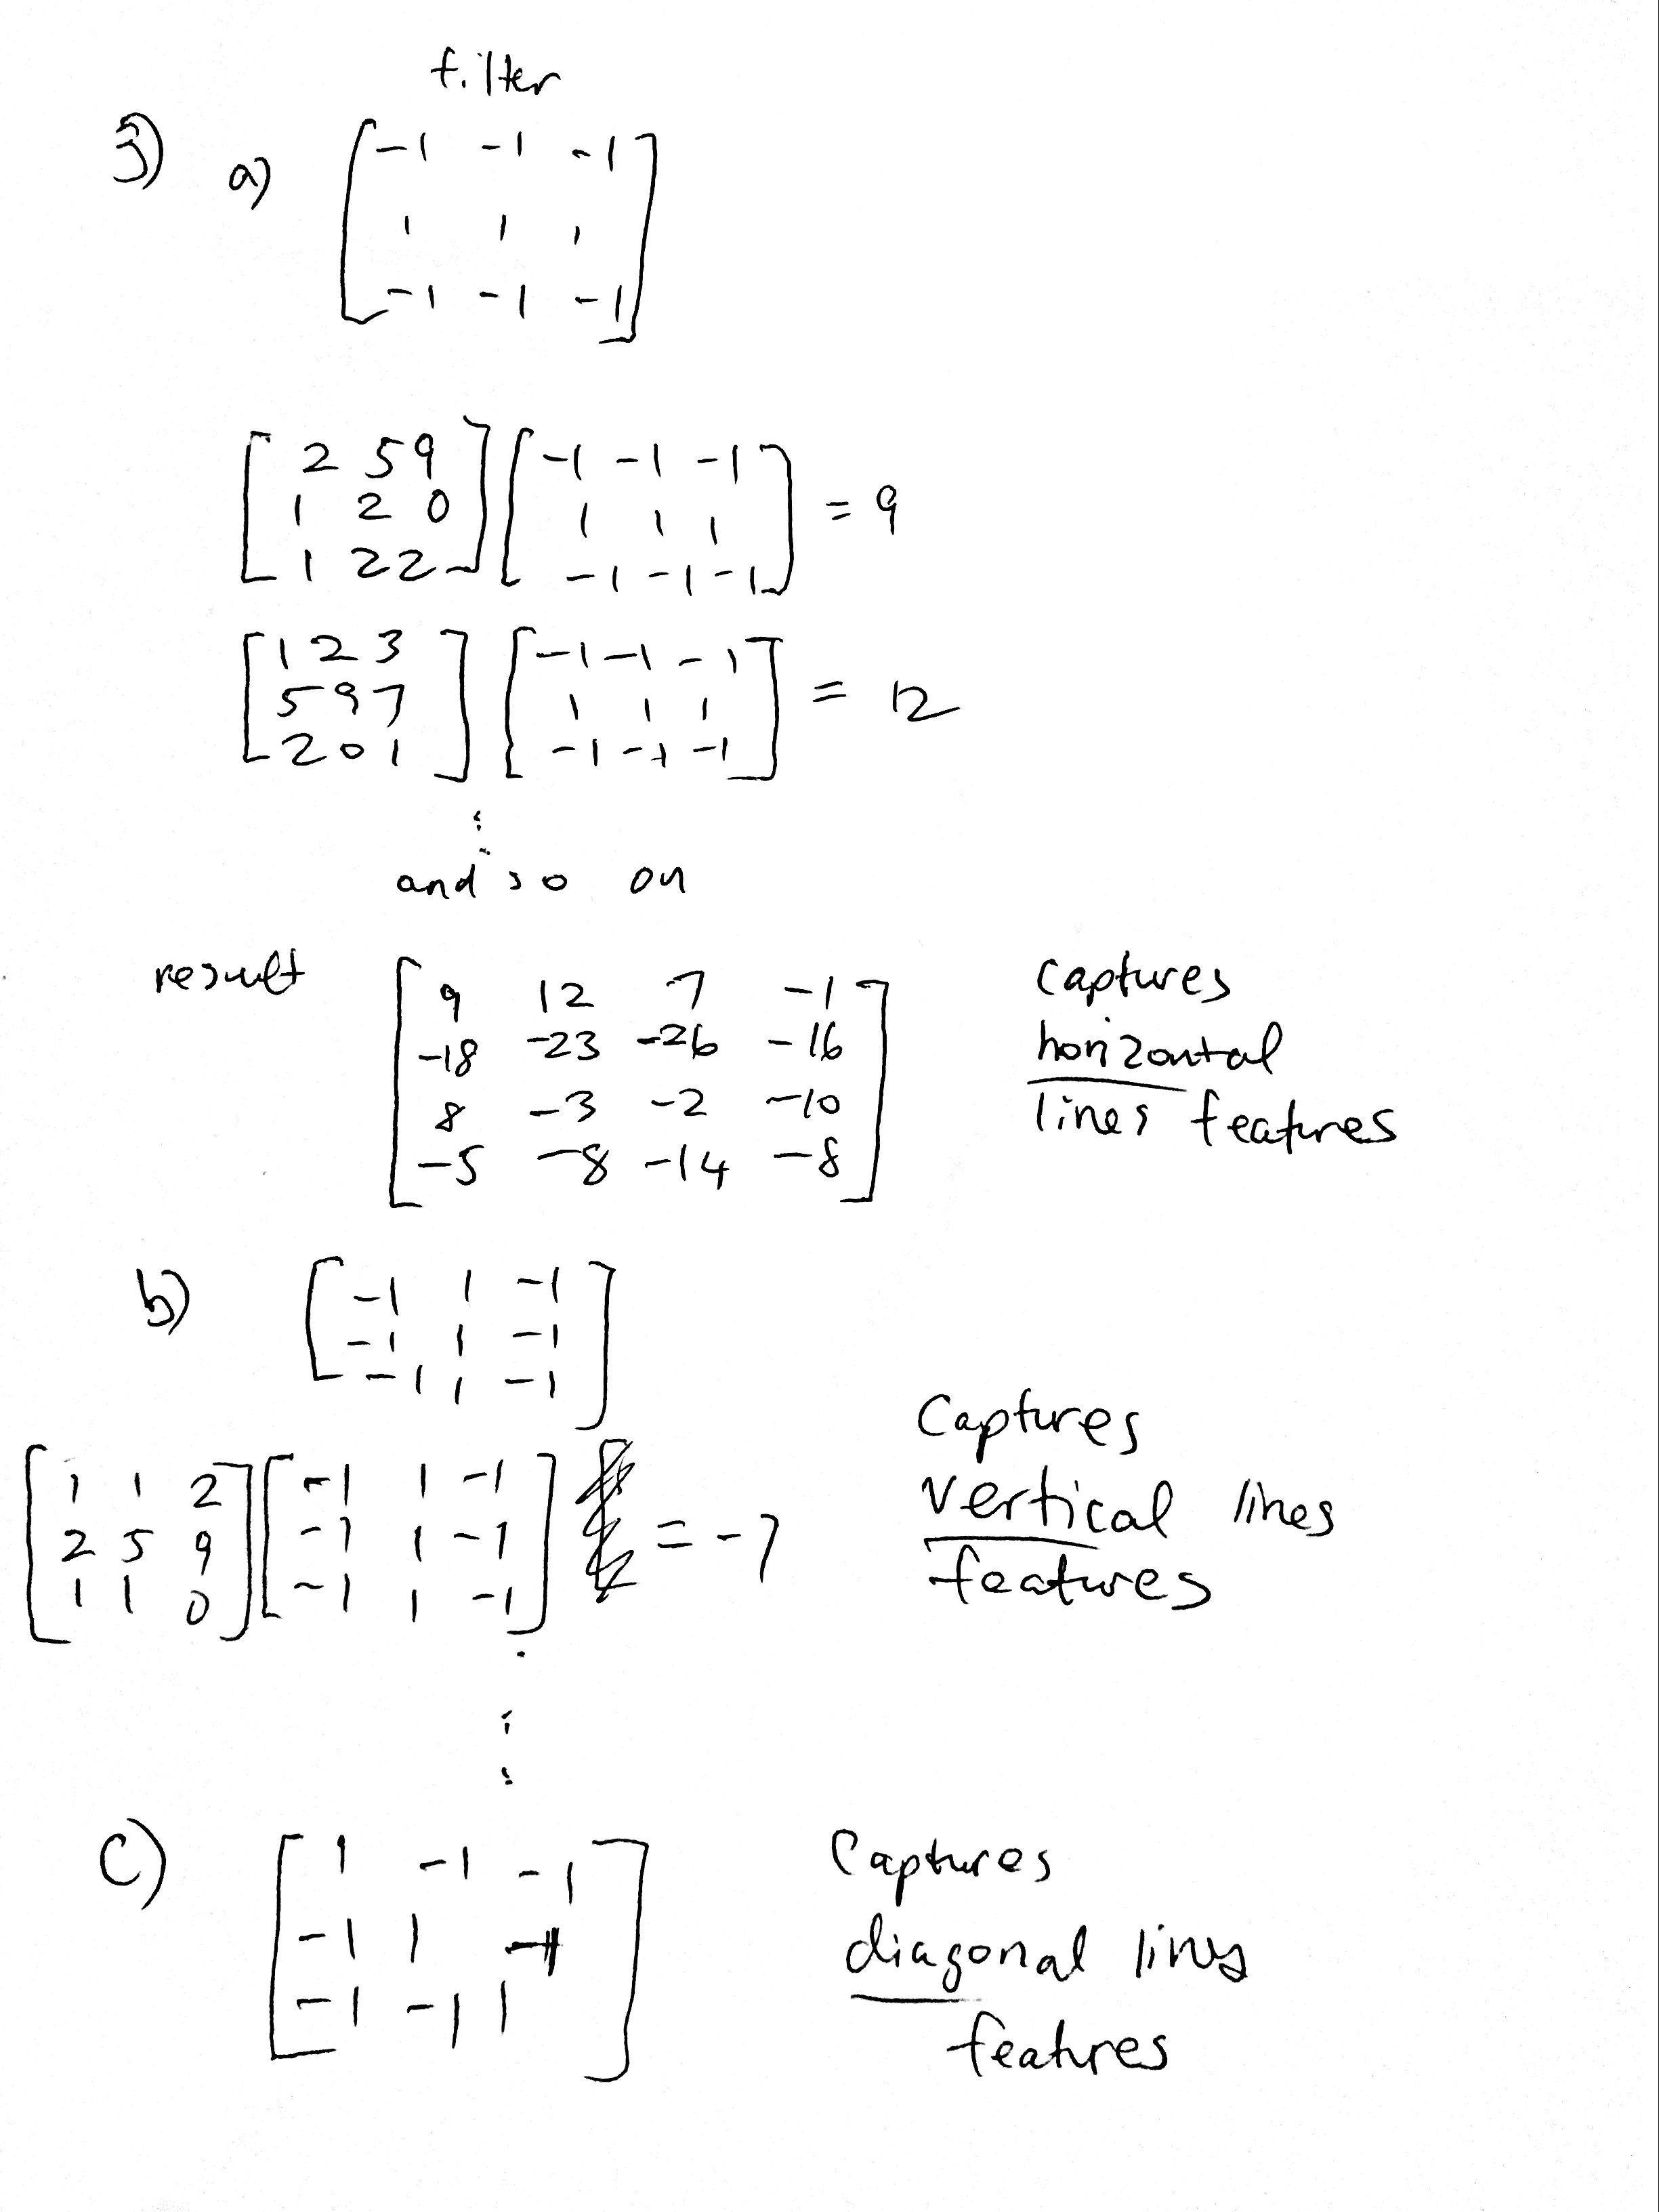
\includegraphics[scale=0.12]{p3} \\ \\ \\ \\ \\ \\ \\ \\ \\ \\

4) \\
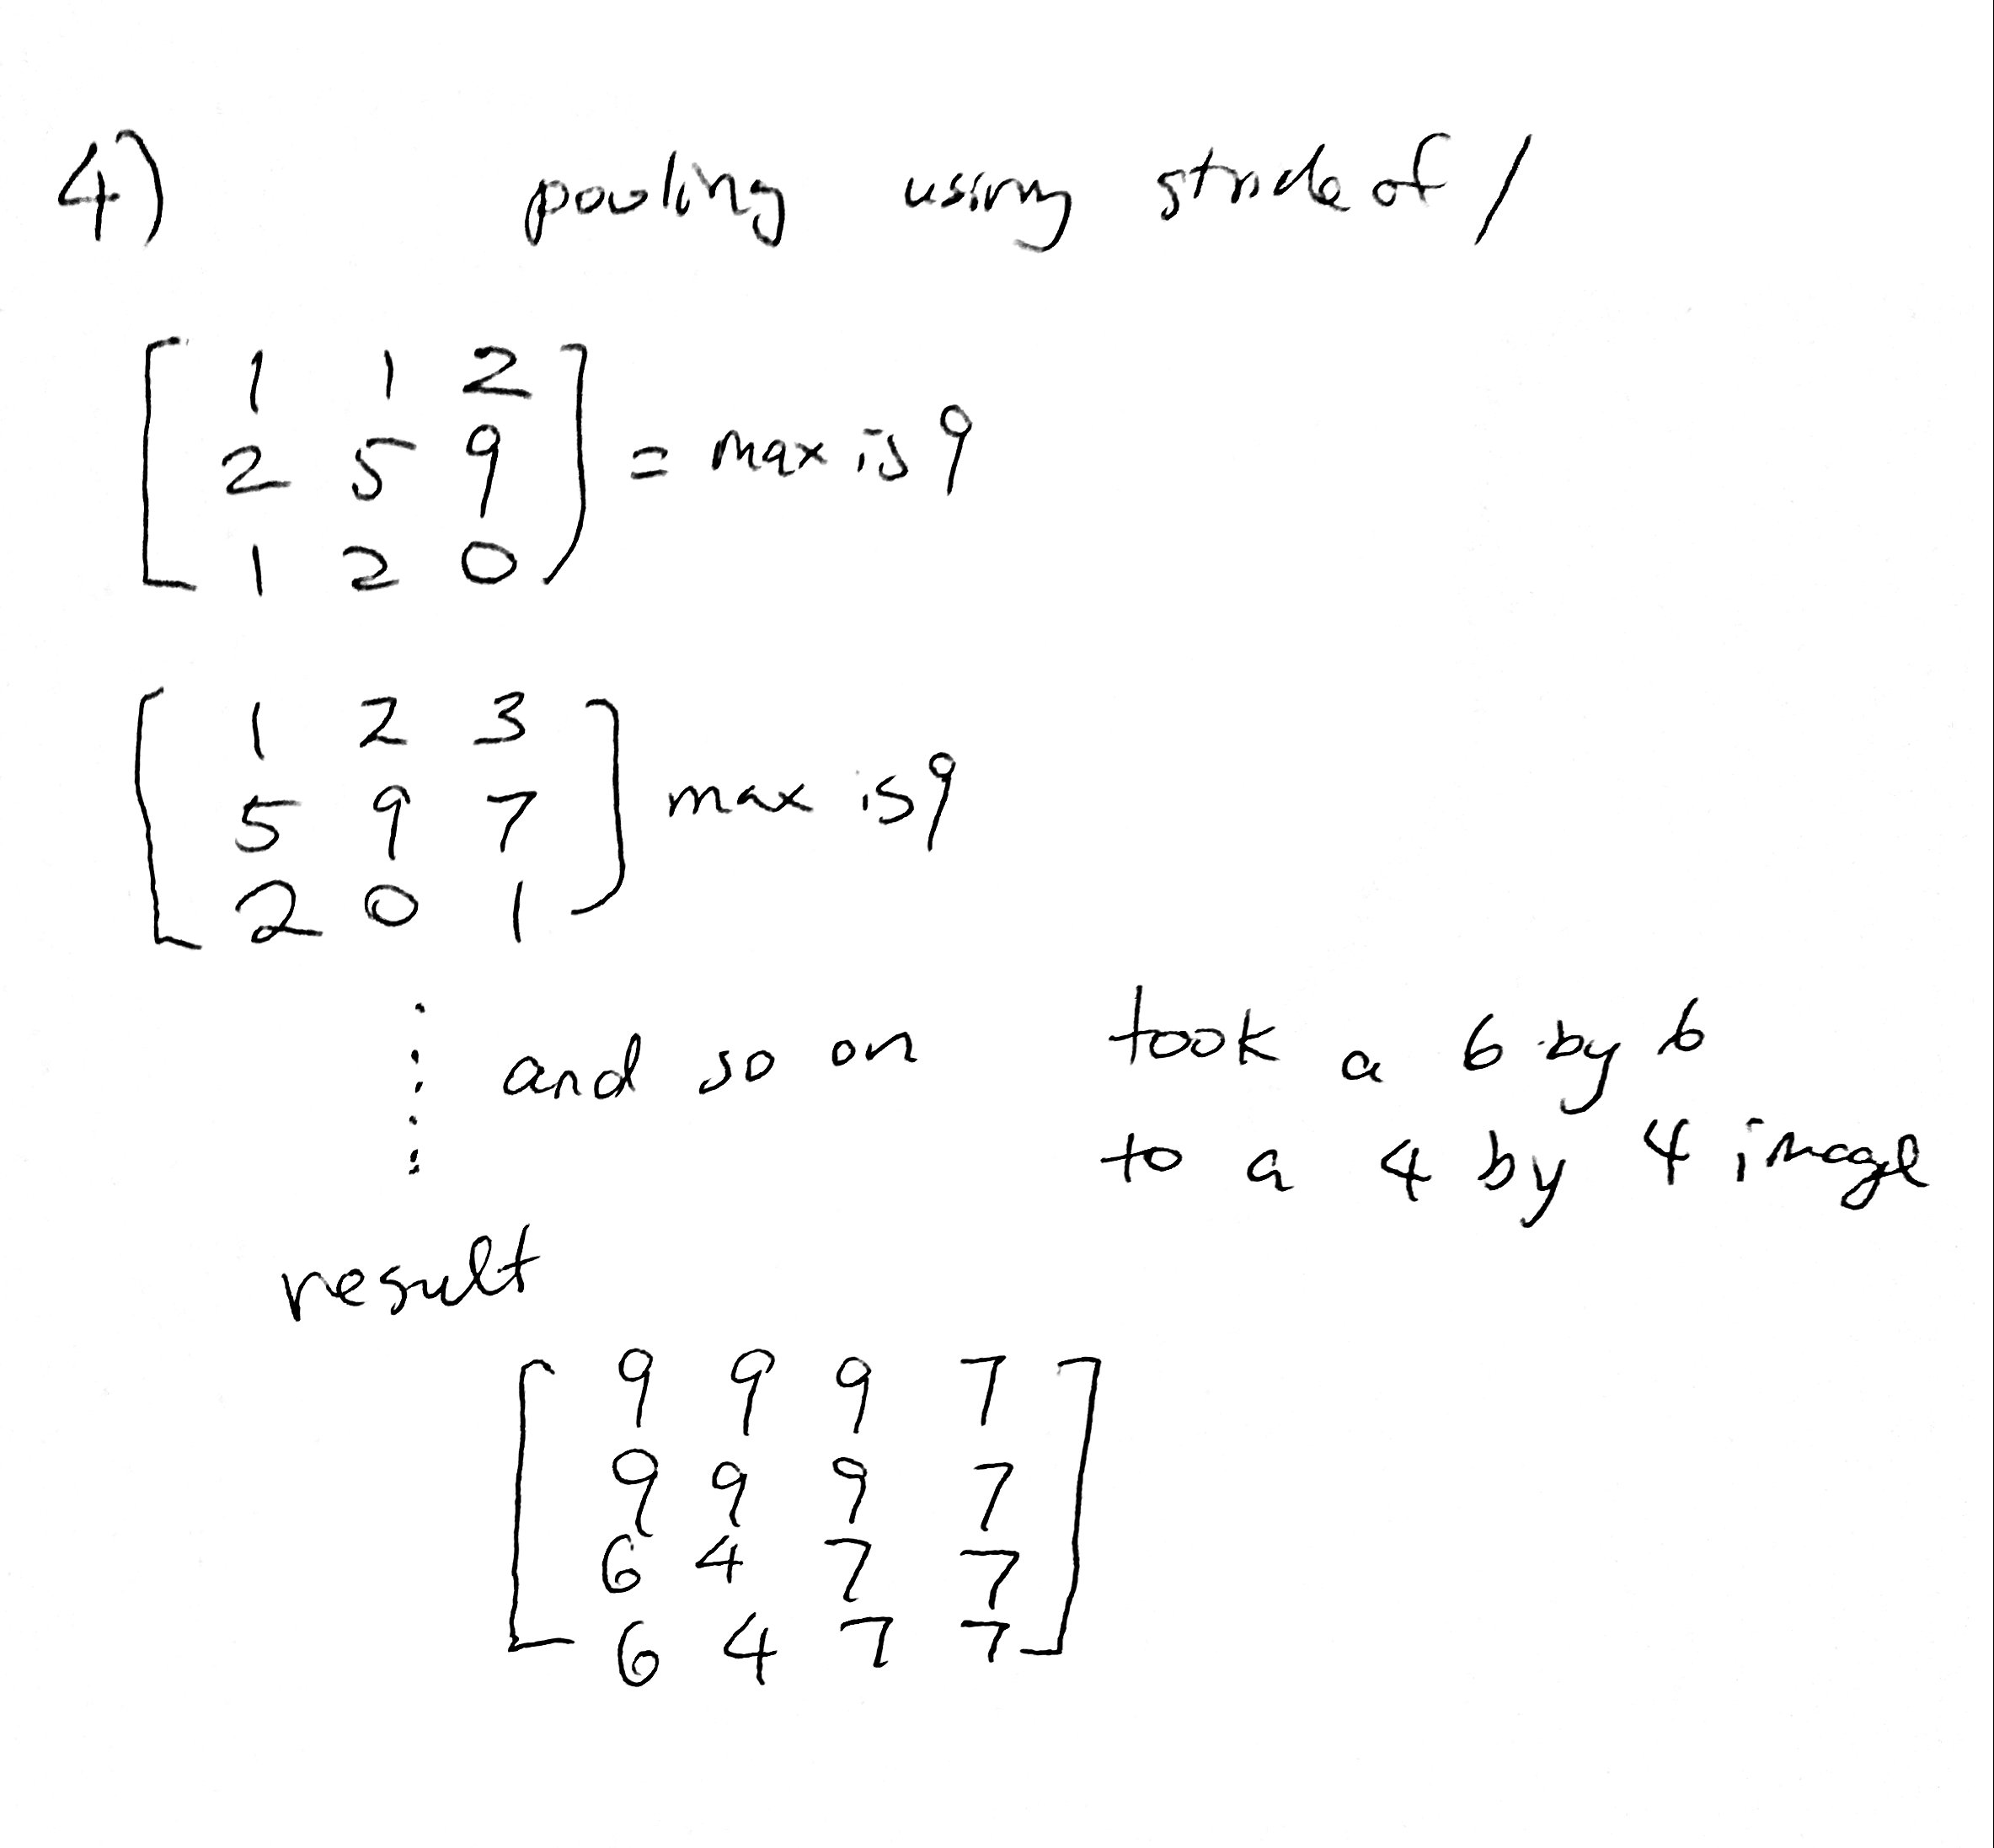
\includegraphics[scale=0.12]{p4}

5) \\
a) 3*4*4 = 48 weights. \\
b) After pooling, there's 3x5x5, so 75 reLu operations performed on the forward pass. \\
c) 48 + 4*75 = 348 weights. \\
d) It seems logical the answer is true. That another neural network with same architecture can represent the same classifier. Not sure how to explain in depth. \\
e) It takes too long to train as there will be too many parameters with fully connected. \\

6) code \\
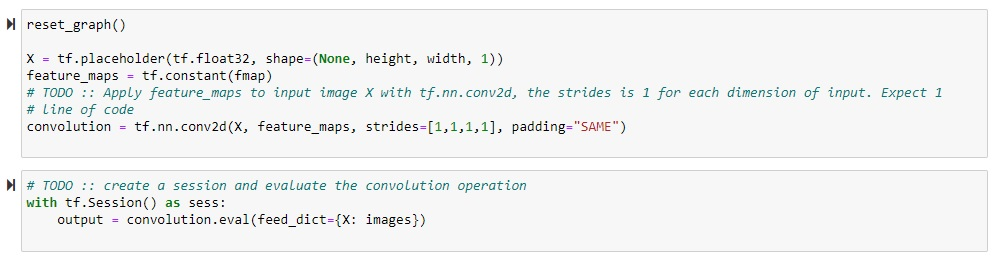
\includegraphics[scale=0.55]{code1} \\
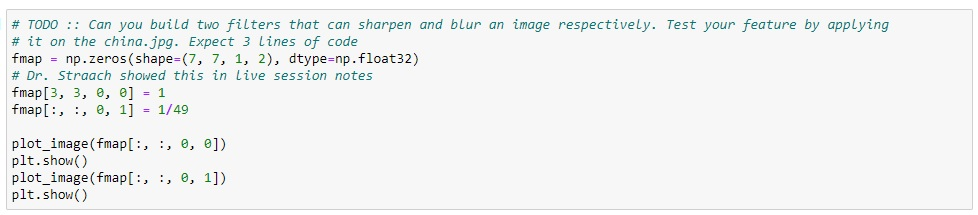
\includegraphics[scale=0.55]{code2} \\
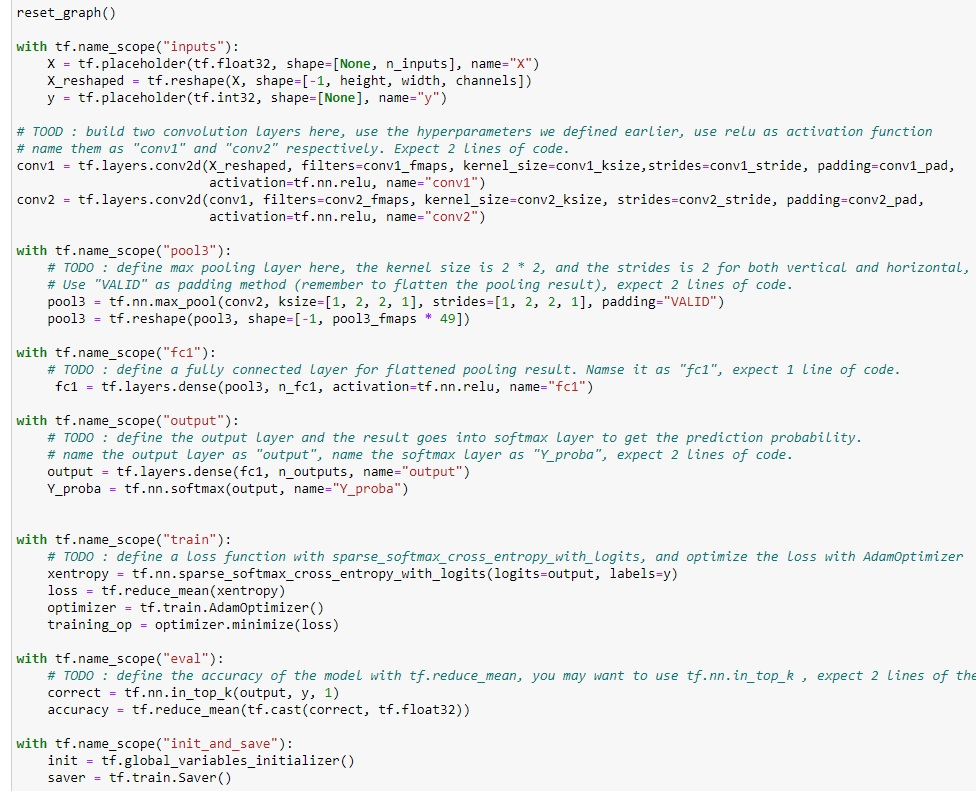
\includegraphics[scale=0.55]{code3} \\
\end{document}

